\documentclass[12pt]{article}

\usepackage{tgtermes}
\usepackage{epsf}
\usepackage{epstopdf}
\usepackage{amsmath}
\usepackage{graphicx}
\usepackage{booktabs}
\usepackage[colorlinks=true,linkcolor=blue,citecolor=blue]{hyperref}
\usepackage{dcolumn}
\usepackage{amsmath, amsthm, amssymb}
\usepackage{mwe}
\usepackage{url}
%\usepackage{harvard}
\usepackage{fancyheadings}
\usepackage{longtable}
\usepackage{authblk}
\usepackage{setspace}
%\usepackage[nomarkers]{endfloat}
\usepackage{float}
\usepackage{bbm}
%\usepackage{titling}
\usepackage{subcaption}
\usepackage{algorithm}
\usepackage{algorithmic}
\usepackage{import}
\usepackage[backend=biber,style=authoryear,
sorting=ynt,citestyle=authoryear]{biblatex}
\addbibresource{papercitations.bib}
%\usepackage[nomarkers,nofiglist,notablist]{endfloat}
\usepackage{subcaption}
\usepackage{caption}

\onehalfspacing
\textwidth 6.5in \oddsidemargin 0in \evensidemargin -0.6in
\textheight 8.5in \topmargin -0.2in

\newcolumntype{L}[1]{>{\raggedright\let\newline\\
		\arraybackslash\hspace{0pt}}m{#1}}
\newcolumntype{C}[1]{>{\centering\let\newline\\
		\arraybackslash\hspace{0pt}}m{#1}}
\newcolumntype{R}[1]{>{\raggedleft\let\newline\\
		\arraybackslash\hspace{0pt}}m{#1}}
\newcolumntype{P}[1]{>{\raggedright\tabularxbackslash}p{#1}}

\newtheorem{theorem}{Theorem}[section]
\newtheorem{corollary}[theorem]{Corollary}
\newtheorem{proposition}[theorem]{Proposition}
\newtheorem{lemma}[theorem]{Lemma}

\captionsetup{justification=centering,singlelinecheck=false}


\newcommand{\xsub}[1]{%
	\mbox{\scriptsize\begin{tabular}{@{}c@{}}#1\end{tabular}}%
}

%\renewcommand{\thetable}{\Roman{table}}

\begin{document}
	
	
	
	
	\linespread{1.2}\title{\vspace{-0.5in} Common Ownership in the Nonprofit Sector:\newline Evidence from the Hospital Industry} 
	
	\date{\today}
	
	\author{\vspace{10mm}Hanna Glenn\footnote{Department of Economics, Emory University, 1602 Fishburne Drive, Atlanta, GA 30322, hanna.glenn@emory.edu.} }
	
	\maketitle
	%\setlength{\droptitle}{-10pt}
	
	\vspace{-0.2in}
	
	\singlespacing\maketitle


 \vspace{3mm}
	
    \begin{abstract}
		{\small

		} 
	\end{abstract}
	
	
	
	
	

	
	\onehalfspacing
	
	\newpage

    \section{Introduction}

    As consolidation in investment companies and in many industries has increased over time, so has the prevalence of common ownership among publicly traded firms. That is, firms within the same industry and market are increasingly owned by the same investment firms. Whether this type of common ownership affects competition is a widely debated theme in the economics literature. Theoretical models predict that common ownership will lead to lower equilibrium output and higher markups through firms placing non-zero weight on competitors' profit (\cite{rubinstein1983competitive}; \cite{rotemberg1984financial}; \cite{azar2012new}). Empirical evidence yields mixed findings, with various studies documenting less competition due to common ownership (\cite{he2017product}; \cite{azar2018anticompetitive}; \cite{azar2022ultimate}; \cite{newham2018common}), but several recent studies that carefully consider identification find either no effect or increased competition due to common ownership (\cite{chen2023does}; \cite{kini2024common}). Additionally, recent literature has considered common ownership in the context of private firms with venture capitalists, where consolidated ownership is even more prevalent, and has found that competition decreases and information sharing increases in this setting (\cite{lindsey2008blurring}; \cite{gonzalez2020exchanges}; \cite{li2023common}; \cite{eldar2024common}). I extend this theme of common ownership and firm behavior to a setting which exhibits similar patterns of affiliation with competing firms in a way that has not yet been considered: board of directors of nonprofits. 

    Unlike publicly traded firms, nonprofits do not have shareholders that receive dividend payments. Instead, the main governing body is a board of directors: a group of volunteers responsible for selecting executives and holding them accountable. In some ways, a board functions similarly to shareholders; they influence the strategic direction of the organization through information sharing and voting on firm decisions without actively managing day-to-day operations. As with investor common ownership, there are no legal restrictions preventing directors from serving on multiple boards, even if those firms are competing in the same industry and market. Therefore, if board members are affiliated with multiple firms and they have the power to influence decisions of the firm, such affiliation might affect firm decisions on product design, output, research and development, and other factors that affect consumers. 
    
    In this paper, I focus specifically on board affiliations among nonprofit hospitals in the US. Nonprofit hospitals play a dominant role in US health care. As of 2023, 50\% of hospitals were private nonprofits, compared to 36\% for-profit. Moreover, nonprofit hospitals operate larger facilities, with an average of 207 staffed beds, compared to 107 in for-profits (\cite{ASPE_2023}). Therefore, nonprofit hospital behavior directly impacts the patient population in the US. Additionally, hospital mergers and consolidations are under increasing scrutiny as competition in the sector has declined significantly in recent years (\cite{levinson2024ten}). It may be that hospital affiliations through board of directors provides a means of informal affiliation that has the power to raise profits but doesn't raise anti-trust concerns. In light of this, the purpose of this paper is two-fold. First, I document the extent of board-level affiliation among plausibly independent nonprofit hospitals, capturing a nonprofit equivalent to common ownership. Second, exploiting timing in board connections formed or lost between hospitals, I explore several potential effects of board affiliations on hospital behavior. While many hospital behaviors are potentially relevant to board member affiliations, I focus specifically on how hospitals with shared board members alter their service offerings and specialization. Board members likely influence hospital decisions through knowledge sharing, which can shape strategic choices about which services to provide or which patient populations to target. This mechanism is particularly relevant if there is asymmetric information about competitors, as hospitals may gain insights from shared board members. 

    To document shared board members of nonprofit hospitals in the US, I compile information on hospital board of director members from publicly available Tax Form 990s, filed each year by nonprofits in the US. One section of this form requires declaration of the names of each member of the board, executives, and highest compensated employees. Extracting these identities and matching to other sources of hospital information, I form a network of hospital board members from 2017-2022. I show that nearly 10\% of the nonprofit hospitals in the sample are affiliated with another hospital through shared board members, even excluding system or network affiliations. Two-thirds of affiliated pairs are made up of two general hospitals, with the remaining pairs consisting of a general hospital affiliated with a specialty hospital. 

    I then construct measures of service offerings and patient populations from two sources of data: the American Hospital Association (AHA) survey, which records the number of beds devoted to a large range of services in each year, and the Center for Medicaid and Medicare Services (CMS) Provider Utilization Files, which record the percent of Medicare patients treated with certain conditions, along with aggregate demographics of Medicare patients seen in the hospital. I construct measures of the concentration of services provided (both in terms of bed allocation and patient percentages) at the hospital-year level using a Herfindahl-Herschmann index calculation, where a highly concentrated hospital specializes in a smaller number of services. I show descriptively that general hospitals unaffiliated through board members have a constant service offering concentration over time, but hospitals with board member affiliations have an increasing service concentration over time. 
    
    To gain a better understanding of the causal effects of shared board member affiliations, I employ a difference-in-differences strategy, comparing hospitals that become affiliated through board members to similar hospitals that do not become affiliated before and after the affiliation begins. Specifically, I employ four different specifications leveraging (1) whether a hospital loses or gains board affiliation with another hospital, and (2) comparison groups of hospitals that are unaffiliated through board, but either belong to a hospital system or not. I estimate the effect of losing or gaining board affiliation on four outcomes: the concentration indexes described above, the total number of Medicare patients seen, and the average risk score of Medicare patients seen. While concentration and risk scores do not seem to affected by board affiliations, the total number of Medicare patients seen increases by 250 patients per year in the second year after becoming affiliated through board members. This indicates potential patient redistribution, possibly through referrals, when more information is gained about competing hospitals. 

    This finding has important implications for hospital competition and patient access to care. If board affiliations facilitate patient redistribution through improved information flow, policymakers should consider how governance structures influence market dynamics. Increased patient volume at affiliated hospitals could improve efficiency and resource allocation, but it may also raise concerns about reduced competition if patient referrals become concentrated within certain networks. To ensure that these affiliations benefit patients without distorting competition, regulators could enhance transparency around board connections and referral practices. 

    This study contributes to the literature on common ownership and firm behavior by examining how shared board affiliations among nonprofit hospitals influence competition and patient distribution. While prior work has largely focused on common ownership in publicly traded firms and venture capital-backed private firms, I extend this line of inquiry to nonprofit hospitals, where governance structures differ but affiliation mechanisms may still shape competitive dynamics. By leveraging a staggered difference-in-differences design, I provide causal evidence on how board affiliations affect hospital service offerings and patient flows, offering novel insights into the role of corporate governance in healthcare markets. [REWRITE THIS TO BE BETTER LATER]

    \section{Data}\label{sec:data}

    
   I compile data on nonprofit hospital board of directors from publicly available Tax Form 990s, which all sufficiently large nonprofits must file with the Internal Revenue Service (IRS) each year. These forms contain a section in which firms declare their board, executives, and highest compensated employees. I limit to firms that have a completed Schedule H in the 990, indicating that the firm runs a hospital. PDF version of the 990s are made public by Nonprofit Explorer dating back earlier than 2009. However, using optical character recognition text extraction algorithms on these PDFs is both time consuming and can lead to small errors in names extracted. Thus, I analyze the data from 2017 onward, when the IRS began publishing XML versions of these files, ensuring more accurate names that can be matched across hospitals and time. I extract all names and positions of individuals listed in the section titled ``Officers, Directors, Trustees, Key Employees, and Five Highest Compensated Employees". I also record information on the hospital that filed the tax form: the Employee Identification Number (EIN), organization name and location, and other characteristics. There are 2,096 hospitals with information extracted directly from the XML files. 

   To observe hospital outcomes regarding service offerings, I must match hospitals in the tax form data to hospitals in other publicly available data sources. The only common information about hospitals across these sources is the name and location. Therefore, I use fuzzy string matching methods to create a crosswalk of EINs to identification numbers in the AHA data. Specifically, I compute the Jaro-Winkler distance between hospital names in each data set. Then, I record matches with a sufficiently small distance and sufficiently similar address. Using this method, I have a sample of 1,623 hospitals in the tax data that can be linked to the AHA survey. From the AHA survey, I gather demographic information about hospitals as well as the allocation of their beds to specific services. Additionally, I merge the CMS Provider Utilization files, which provides hospital-level information about the types of Medicare patients seen in each year, including percent of patients of a certain race or age, and the percent of patients treated for specific conditions.

    Next, I clean the column of board member names by removing common titles (Dr., Reverand, etc.), and combining names within the same firm that have slight spelling differences. For example, if John Matthews is a board member of hospital A in 2017, and John Mathews is a board member of hospital A in 2018, I assume these names represent the same person. Additionally, I combine names within the same HRR that are identical apart from small mis-characters such as the presence of a middle initial. Finally, to avoid issues in whether first or last names are listed first, I sort each individual's names alphabetically. I define a hospital as being affiliated if the same individual is a board member of two otherwise unaffiliated hospitals. That is, two hospitals that do not belong to the same system or network can be affiliated through board members, but same-system or same-network hospitals can not. I make this distinction to separate the variation in affiliation by board member alone versus simply having shared board members due to being in the same system, which is plausibly already correlated with service offerings. I also focus on affiliations within the same hospital market, as the outcomes of interest focus on competing for patients in a specific geographic region. I measure hospital markets using Hospital Referral Regions (HRRs) as defined by Dartmouth Atlas of Healthcare.

    \import{Objects}{all_summarystats.tex}
    


    \section{Documenting Board of Director Affiliation}


    Of the approximately 1400 hospitals in the final sample, approximately 7\% are affiliated with another hospital through a shared board member. As shown in Figure \ref{fig:connected_percent}, this percentage remains relatively constant over time, decreasing from 132 affiliated hospitals in 2017 to 117 affiliated hospitals in 2021. 

    \begin{figure}[ht!]
        \centering
        \caption{Percent of hospitals that have a board affiliation}
        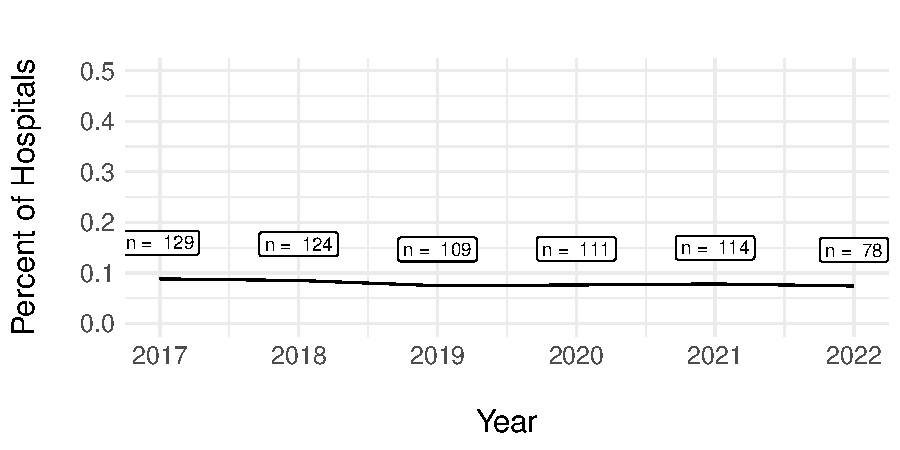
\includegraphics[width=.8\textwidth]{Objects/connected_percent.pdf}
        \label{fig:connected_percent}
    \end{figure}

    As mentioned previously, common board members should be more likely to affect behavior within a hospital market, where hospitals compete for the same patient population. Of the 306 HRRs in the US, approximately 17\% have at least one pair of board affiliated hospitals within the market. As shown in Figure \ref{fig:connected_HRR_percent}, this proportion decreases slightly over time, with 15\% of HRRs having connected hospitals in 2021, a nominal decrease of 8 markets losing hospitals with affiliation.  


    \begin{figure}[ht!]
        \centering
        \caption{Percent of HRRs containing board affiliated hospitals}
        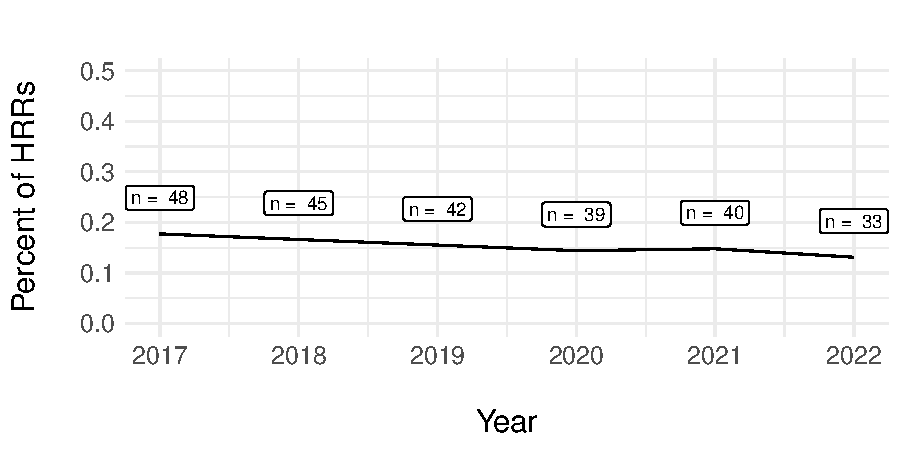
\includegraphics[width=.8\textwidth]{Objects/connected_HRR_percent.pdf}
        \label{fig:connected_HRR_percent}
    \end{figure}

    The geographic distribution of these pairs is shown in Figure \ref{fig:connected_maps}, where the blue dots represent hospitals that share a common board member. Connected hospitals are distributed fairly regularly across the US, apart from relatively few connections on the west coast relative to the population. Over time, the connections remain fairly consistent geographically.

    \begin{figure}[ht!]
        \centering
        \caption{Geographic distribution of board affiliated hospitals over time}
        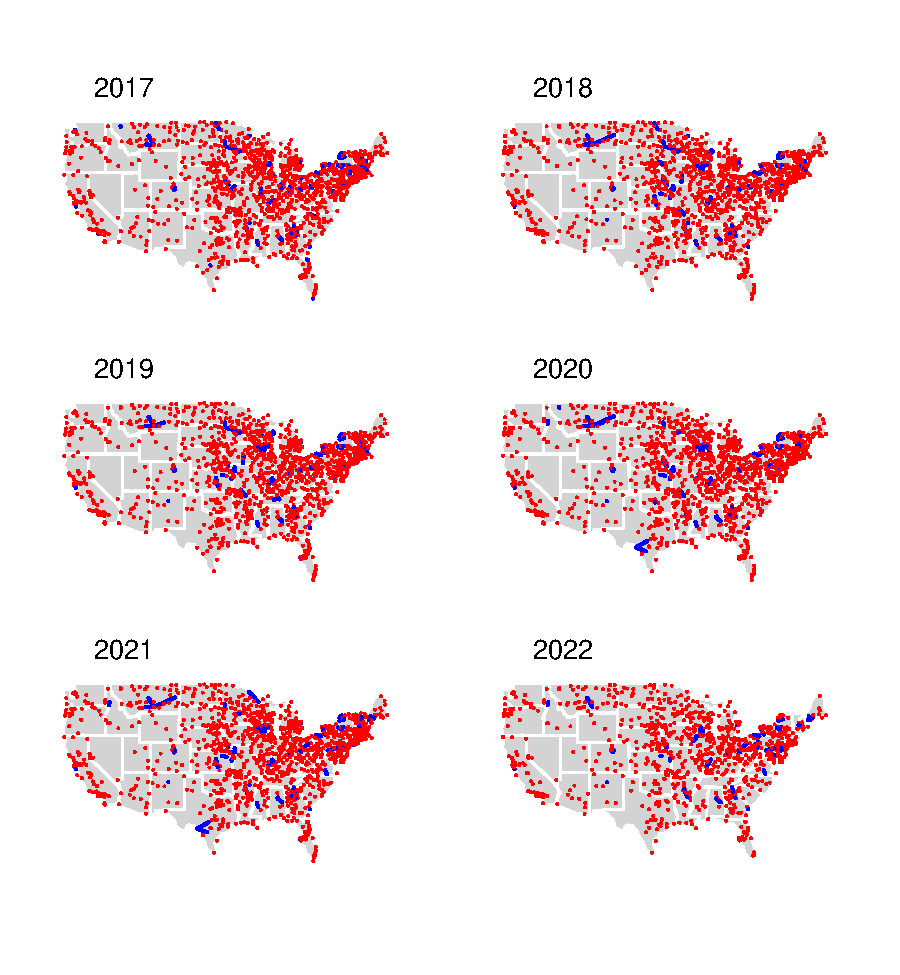
\includegraphics[width=.8\textwidth]{Objects/connected_maps.pdf}
        \label{fig:connected_maps}
    \end{figure}



    Next, I show the proportion of the type of hospital affiliations in Table \ref{tab:hospital_pair_types}. Each hospital is general or specialty, children or adult, and independent or system, all characteristics found in the AHA data. Two-thirds of board affiliated pairs are between two general hospitals, and 10\% of pairs are between a specialty and a general hospital. In the main analysis, I focus only on the affiliations between general hospitals, as this is the most prominent pair type and the most direct competition. 
    There is also significant variation in the ownership type of pairs. Forty-five percent of pairs are between two non-system affiliated hospitals, and 36\% of pairs are between an independent hospital affiliated with a hospital belonging to a system. In total, there are 217 hospitals that are affiliated with at least one other hospital through shared board members at some point in the sample. 

    \import{Objects}{hospital_pair_types.tex}

    I now shift towards examining summary statistics of hospitals with different types of affiliation relationships. First, in Table \ref{tab:hospital_general_summarystats}, I focus on general hospitals in four categories: affiliated through shared board members with another general hospital, affiliated through shared board members with a specialty hospital, unaffiliated through board members but belonging to a system, and completely unaffiliated. I present means of hospitals in each of these categories for the number of beds, the number of patients seen, whether it is an academic medical center, and whether the hospital is located in a metropolitan area. On these dimensions, hospitals affiliated with other general hospitals (column 1) are relatively similar to unaffiliated hospitals that are part of a system (column 3). Unaffiliated hospitals that are not part of a system are slightly smaller in terms of bed size and number of patients seen, and less likely to be in a metropolitan area. The hospitals in column (2) are outliers, with a large number of beds and patients seen, and mainly in metropolitan areas. There are only 12 hospitals in this sample that are likely very different from the average general hospital. 

    \import{Objects}{hospital_general_summarystats.tex}

    I also present means of variables to capture aspects of the service offerings of the different types of hospitals. First, from the AHA survey, I include an indicator for whether the hospital offers services in a Neonatal Intensive Care Unit (NICU) or Cardiac catheterization lab, both specialized and profitable services. General hospitals that are affiliated with specialty hospitals are the most likely to offer these services. Hospitals without any board member affiliations but belonging to a system are more likely to offer these services than unaffiliated hospitals that do not belong to a system. Hospitals that are affiliated with another general hospitals fall somewhere in between these two, with slightly less likelihood than the unaffiliated hospitals belonging to a system. I also include a measure of the concentration of services offered by the hospital using a Herfindahl-Hirschman Index calculation of the number of beds devoted to each service category in the AHA data. Specifically, for each hospital, I compute the proportion of total beds assigned to each service category and then square these proportions before summing them. A higher HHI value indicates that a hospital's bed capacity is concentrated in fewer service categories, whereas a lower HHI suggests a more diversified service offering, which provides insight into the degree of specialization or diversification in a hospital’s service provision. I also compute a similar concentration metric using the percent of patients in several service categories from the CMS Provider Utilization Files, including cancer, Chronic Obstructive Pulmonary Disease (COPD), kidney, and heart-related services. For both measures, there seems to be little variation in service concentration across affiliation types.

    Next, I present the same summary statistics for specialty hospitals with different types of affiliations: affiliated with a general hospital, unaffiliated through board but belonging to a system, and unaffiliated through board or system, shown in Table \ref{tab:hospital_specialty_summarystats}. Overall, there are less specialty hospitals included in the sample, and very few of them are affiliated through board members. Specialty hospitals are more concentrated than general hospitals, as expected. In the AHA measure of concentration, all specialty hospitals are similarly concentrated. However, when using the services included in the CMS files, the concentration of unaffiliated system hospitals is much lower than that of any other specialty hospital. This could be due to the limited services included in the CMS data. 

    \import{Objects}{hospital_specialty_summarystats.tex}

    In Figure \ref{fig:concentration_services_time}, I show the AHA measure of service concentration based on the number of beds over time for general hospitals with different levels of affiliation. General hospitals that are unaffiliated through board members, whether they are affiliated with a system or not, remain relatively constant in their service offerings over time. However, general hospitals that are affiliated with another general hospital through a shared board member display increasing service concentration over time, suggesting that there may be some correlation between board affiliations and the services offered in hospitals.  

    \begin{figure}[ht!]
        \centering
        \caption{Concentration of services offered over time}
        \includegraphics[width=0.8\textwidth]{Objects/concentration_services_time.pdf}
        \label{fig:concentration_services_time}
    \end{figure}


    \section{Effect of Board Affiliation on Hospital Services and Patients}

    I estimate the average effect of either losing or gaining board affiliation on the outcomes discussed in Section \ref{sec:data} using a staggered timing difference in differences strategy. For simplicity, I only consider general hospitals in both the treatment and control groups, as they are the majority of connections and the most closely related competitors within a market. Further, I leverage the variation in different types of affiliation, whether via board members or system ownership, by defining separate control groups of unaffiliated hospitals into system or non-system categories. Therefore, I define four relevant subsets of hospitals. First, I construct two groups of ``treated" hospitals, where treatment is defined as either losing an established board affiliation for the remainder of the time period, or gaining a shared board affiliation that remains for the rest of the time period. After dropping hospitals that lose or gain affiliation multiple times, there are 112 hospitals who are affiliated at some point, 59 0f which lose affiliation at some point and 53 of which gain affiliation at some point. Then, I define two ``control" groups of hospitals, those that are a part of a formal hospital system or not. 

    Since hospitals can lose or gain affiliated board members at different times, negative weighting issues can arise when employing a classic two way fixed effects specification. Thus, I estimate average treatment effects for a specific group $g$ at time $t$:
    
    $$ATT(g,t)=\mathbbm{E}[Y_t(g)-Y_t(0)|G_g=1],$$
    
    \noindent where $G_g=1$ for those in group $g$. A group represents hospitals that are treated, defined as gaining or losing board affiliation, in the same year. I employ the doubly robust estimator established in \citeauthor{sant2020doubly} (\citeyear{sant2020doubly}). I aggregate the group-time estimates into a more conventional event study plot, incorporating simultaneous confidence bands derived from bootstrapped standard errors. 

    There are several necessary assumptions to identify the parameters of interest, $ATT(g,t)$. First, I assume that once a hospital gains or loses board affiliation with another hospital, this affiliation is not reversed. I ensure this mechanically by only including hospitals in the treated sample who establish or lose a board affiliation once for the entire time period. Second, I assume there is no anticipation of treatment. That is, hospitals do not change behavior based on the expectation of gaining or losing board affiliation. As is usual in a difference-in-differences framework, I also assume a version of parallel trends based on never-treated units. I assume that average outcomes for hospitals treated in group $g$ would have followed a parallel trend as hospitals that were never board affiliated in the absence of treatment. 

    \subsection{Concentration of Bed Allocation}

    In Figure \ref{fig:aha_hhi_did}, I present the estimated effect of either losing board affiliation or gaining board affiliation with another hospital on the concentration of bed allocation. As described in Section \ref{sec:data}, I construct this concentration measure using the number of beds a hospital allocates towards different services. While the magnitude itself does not have a direct interpretation, relative magnitudes indicate more or less specialized hospitals. 

    \begin{figure}[ht!]
        \centering
        \caption{Effect of Board Affiliation on Concentration of Bed Allocation}
        \includegraphics[width=0.75\textwidth]{Objects/aha_hhi_did.pdf}
        \label{fig:aha_hhi_did}
    \end{figure}

    The top panel of Figure \ref{fig:aha_hhi_did} compares hospitals who lose a board affiliation at some point in time with hospitals who never had a board affiliation, and the bottom panel compares hospitals who gain a board affiliation to hospitals that never have an affiliation. Relative time $t=0$ is the point at which shared board members were gained or lost. In yellow, the comparison group contains hospitals that do not belong to a system. In gray, the comparison group contains hospitals that do belong to a system but are unaffiliated by board members outside of their system. In all specifications, there is no statistically significant difference between board affiliated and non-board-affiliated hospitals in terms of how specialized their bed allocation is. It could be that this measure of service offerings is sticky in the short run, and that hospitals do not make drastic changes to their bed allocations. However, even with constant bed allocations, the types of patients that a hospital treats might change in the short run. 

    \subsection{Concentration of Patient Treatment}

    A more adjustable measure in the short run could be patient-driven specialization as opposed to bed allocation. The type of patients seen in the hospital can be altered by referral patterns, patient demand, or advertising. Therefore, I now present the effect of losing or gaining board affiliation on the concentration of patients seen for specific conditions. The calculation is similar to how I constructed the bed allocation measure, although I now calculate the HHI index using the share of patients treated for various conditions, as described in Section \ref{sec:data}. I present the estimated average treatment effects in Figure \ref{fig:cms_hhi_did}. 

    \begin{figure}[ht!]
        \centering
        \caption{Effect of Board Affiliation on Concentration of Patient Treatment}
        \includegraphics[width=0.75\textwidth]{Objects/cms_hhi_did.pdf}
        \label{fig:cms_hhi_did}
    \end{figure}

    I compare hospitals who lose board affiliation to those who were never affiliated in the top panel of Figure \ref{fig:cms_hhi_did}. There is slight evidence that hospitals who lose board affiliation have relatively more concentrated patient services than unaffiliated hospitals, although the magnitude is quite small relative to the mean patient concentration of around .5. Additionally, there is no effect of gaining board affiliation on patient treatment concentration, shown in the bottom panel of Figure \ref{fig:cms_hhi_did}. These results, taken with the null effect on the bed allocation concentration, indicate that the services offered to patients do not change much as a result of shared board members. 

    \subsection{Medicare and Medicaid Patients}

    A common outcome studied in the common ownership literature is output. In hospitals, output is roughly equivalent to the patients treated in the hospital. However, there are differences in the types of patients a hospital can treat. Private patients are the most profitable, and therefore the most desirable to hospitals, while publicly insured patients are often seen as less profitable. Thus, board affiliations might affect the flow of different types of patients seen in different hospitals. For example, a hospital might direct patient referrals to a board-affiliated hospital over a hospital they have no affiliation with. Therefore, I consider three outcomes of patient composition that I observe in the AHA or CMS data. First, I show the effect of losing or gaining common ownership on the total number of Medicare patients seen in the hospital from the CMS Provider Utilization Files in Figure \ref{fig:benes_did}. 
    

    \begin{figure}[ht!]
        \centering
        \caption{Effect of Board Affiliation on Number of Medicare Patients}
        \includegraphics[width=0.75\textwidth]{Objects/benes_did.pdf}
        \label{fig:benes_did}
    \end{figure}

    The top panel of Figure \ref{fig:benes_did} shows the relative change of the number of Medicare patients when a hospital loses board affiliation. In yellow, the comparison group consists of non-system hospitals. In gray, the comparison group consists of hospitals belonging to systems. There is a slight increase in Medicare patients for hospitals losing affiliation compared to system hospitals, but this magnitude is small and only persists for one year. However, the bottom panel shows that hospitals that gain a board affiliation have an increased number of Medicare patients compared to non-system, non-board-affiliated hospitals in both the second and third year after becoming board affiliated. This magnitude of approximately 250 additional Medicare patients is meaningful compared to the average number of Medicare patients, approximately 3,000. This increase indicates a potential change in patient volume or patient composition once a hospital becomes affiliated through board members. 

    To dig into this a little deeper, I also estimate the effect of gaining or losing board affiliation on Medicare and Medicaid discharges relative to the total number of beds in the hospital. 

    \begin{figure}[ht!]
        \centering
        \caption{Effect of Board Affiliation on Medicare/Bed}
        \includegraphics[width=0.75\textwidth]{Objects/mcare_did.pdf}
        \label{fig:mcare_did}
    \end{figure}

    \begin{figure}[ht!]
        \centering
        \caption{Effect of Board Affiliation on Medicaid/Bed}
        \includegraphics[width=0.75\textwidth]{Objects/mcaid_did.pdf}
        \label{fig:mcaid_did}
    \end{figure}

    While not a perfect measure of patient volume, this measure will give an indication of whether total volume or the types of patients a hospital admits might change due to board affiliation. 

    \subsection{Risk Score of Medicare Patients}

    Finally, I present estimates of how board affiliation affects the average risk score of patients in the hospital in Figure \ref{fig:risk_did}. A higher risk score indicates that patients seen in that hospital have, on average, more complex conditions. This outcome might indicate whether patient composition changes as a result of board affiliation. 

    \begin{figure}[ht!]
        \centering
        \caption{Effect of Board Affiliation on Risk Score}
        \includegraphics[width=0.75\textwidth]{Objects/risk_did.pdf}
        \label{fig:risk_did}
    \end{figure}

    Again, the top panel of Figure \ref{fig:risk_did} includes the sample of hospitals who lose their board affiliation at some point as the treated group and hospitals who were never board affiliated as the comparison group. The comparison group is also divided into those who belong to a system, in gray, and those who do not belong to a system, in yellow. Hospitals that lose their board affiliation have a slight increase in the risk score of their Medicare patients after losing board affiliation relative to both types of comparison hospitals. For non-system hospitals, this happens in the first year after losing affiliation, whereas for system hospitals this happens in the second year. However, this increase in risk score might indicate that losing affiliation affects the patients coming through the hospital, potentially through referrals. Interestingly, the bottom panel of Figure \ref{fig:risk_did} shows that hospitals who gain board affiliation also have an increased risk score relative to the comparison non-system hospitals. [EXPLANATION??]

    

    \newpage


    \printbibliography


    

    

    

    

    

	
	
	


\end{document}

